\chapter[GLM]{Generalized Linear Models}

\begin{objetivos}
By the end of this chapter, readers should understand generalized linear models
(GLMs) in SDM; fit presence--background models with a binomial family;
interpret coefficients and linear and quadratic terms; assess predictive
performance using AUC and TSS; generate partial response curves; project
environmental suitability into geographic space; and map current suitability
for \textit{Dinizia excelsa} across the Amazon biome.
\end{objetivos}

\section{Introduction}

Generalized linear models are among the most established and interpretable
statistical approaches in species distribution modeling. They commonly relate
presence--absence or presence--background observations to environmental
predictors \parencite{guisan2000,guisan2005predicting,guisan2017habitat}.

In a presence--background model, presences are coded 1 and background points 0.
Background points are not confirmed absences; they represent the environmental
conditions available within the calibration area. With background coded as the
contrast class, the fitted GLM estimates a relative occurrence or environmental
suitability score along the environmental gradients, not an absolute occurrence
probability.

\begin{conceito}[title={\faBook\quad GLMs in SDM}]
A binomial GLM uses a logit link to relate species occurrence to environmental
variables, transforming a linear predictor into values between 0 and 1.
\end{conceito}

\section{Mathematical Formulation}

For the binomial case, let $Y_i$ indicate presence or background:

\[
Y_i =
\begin{cases}
  1, & \text{presence},\\
  0, & \text{background}.
\end{cases}
\]

The GLM with a logit link is

\begin{equationbox}
\[
\operatorname{logit}(p_i)=
\log\left(\frac{p_i}{1-p_i}\right)
=\beta_0+\beta_1X_{1i}+\beta_2X_{2i}+\cdots+\beta_kX_{ki},
\]
\[
p_i=\frac{1}{1+\exp(-\eta_i)}.
\]
\end{equationbox}

Here, $p_i$ is estimated suitability in pixel $i$, $X_k$ denotes the
environmental predictors, and $\beta_k$ denotes estimated coefficients.

\begin{dica}[title={\faLightbulb\quad Quadratic terms}]
Quadratic terms allow unimodal responses in which suitability is greatest at
intermediate values of an environmental variable.
\end{dica}

\section{Preparing Data for the GLM}

The presence--background dataset from Chapter 5 is used here. Presences are the
final \textit{Dinizia excelsa} records, and background points were sampled
within the accessible area $M$. Together they form the calibration dataset.

\rscriptfile{scripts/unidade06/01_estrutura_pastas.R}
\rscriptfile{scripts/unidade06/02_preparar_dados_glm.R}

\section{Fitting the GLM}

The model uses a binomial family and logit link. Linear and quadratic terms
increase ecological flexibility. Before fitting, predictors are standardized
to zero mean and unit standard deviation, reducing numerical problems and
facilitating coefficient comparisons.

\rscriptfile{scripts/unidade06/03_ajustar_glm_dinizia.R}

\begin{figure}[H]
  \centering
  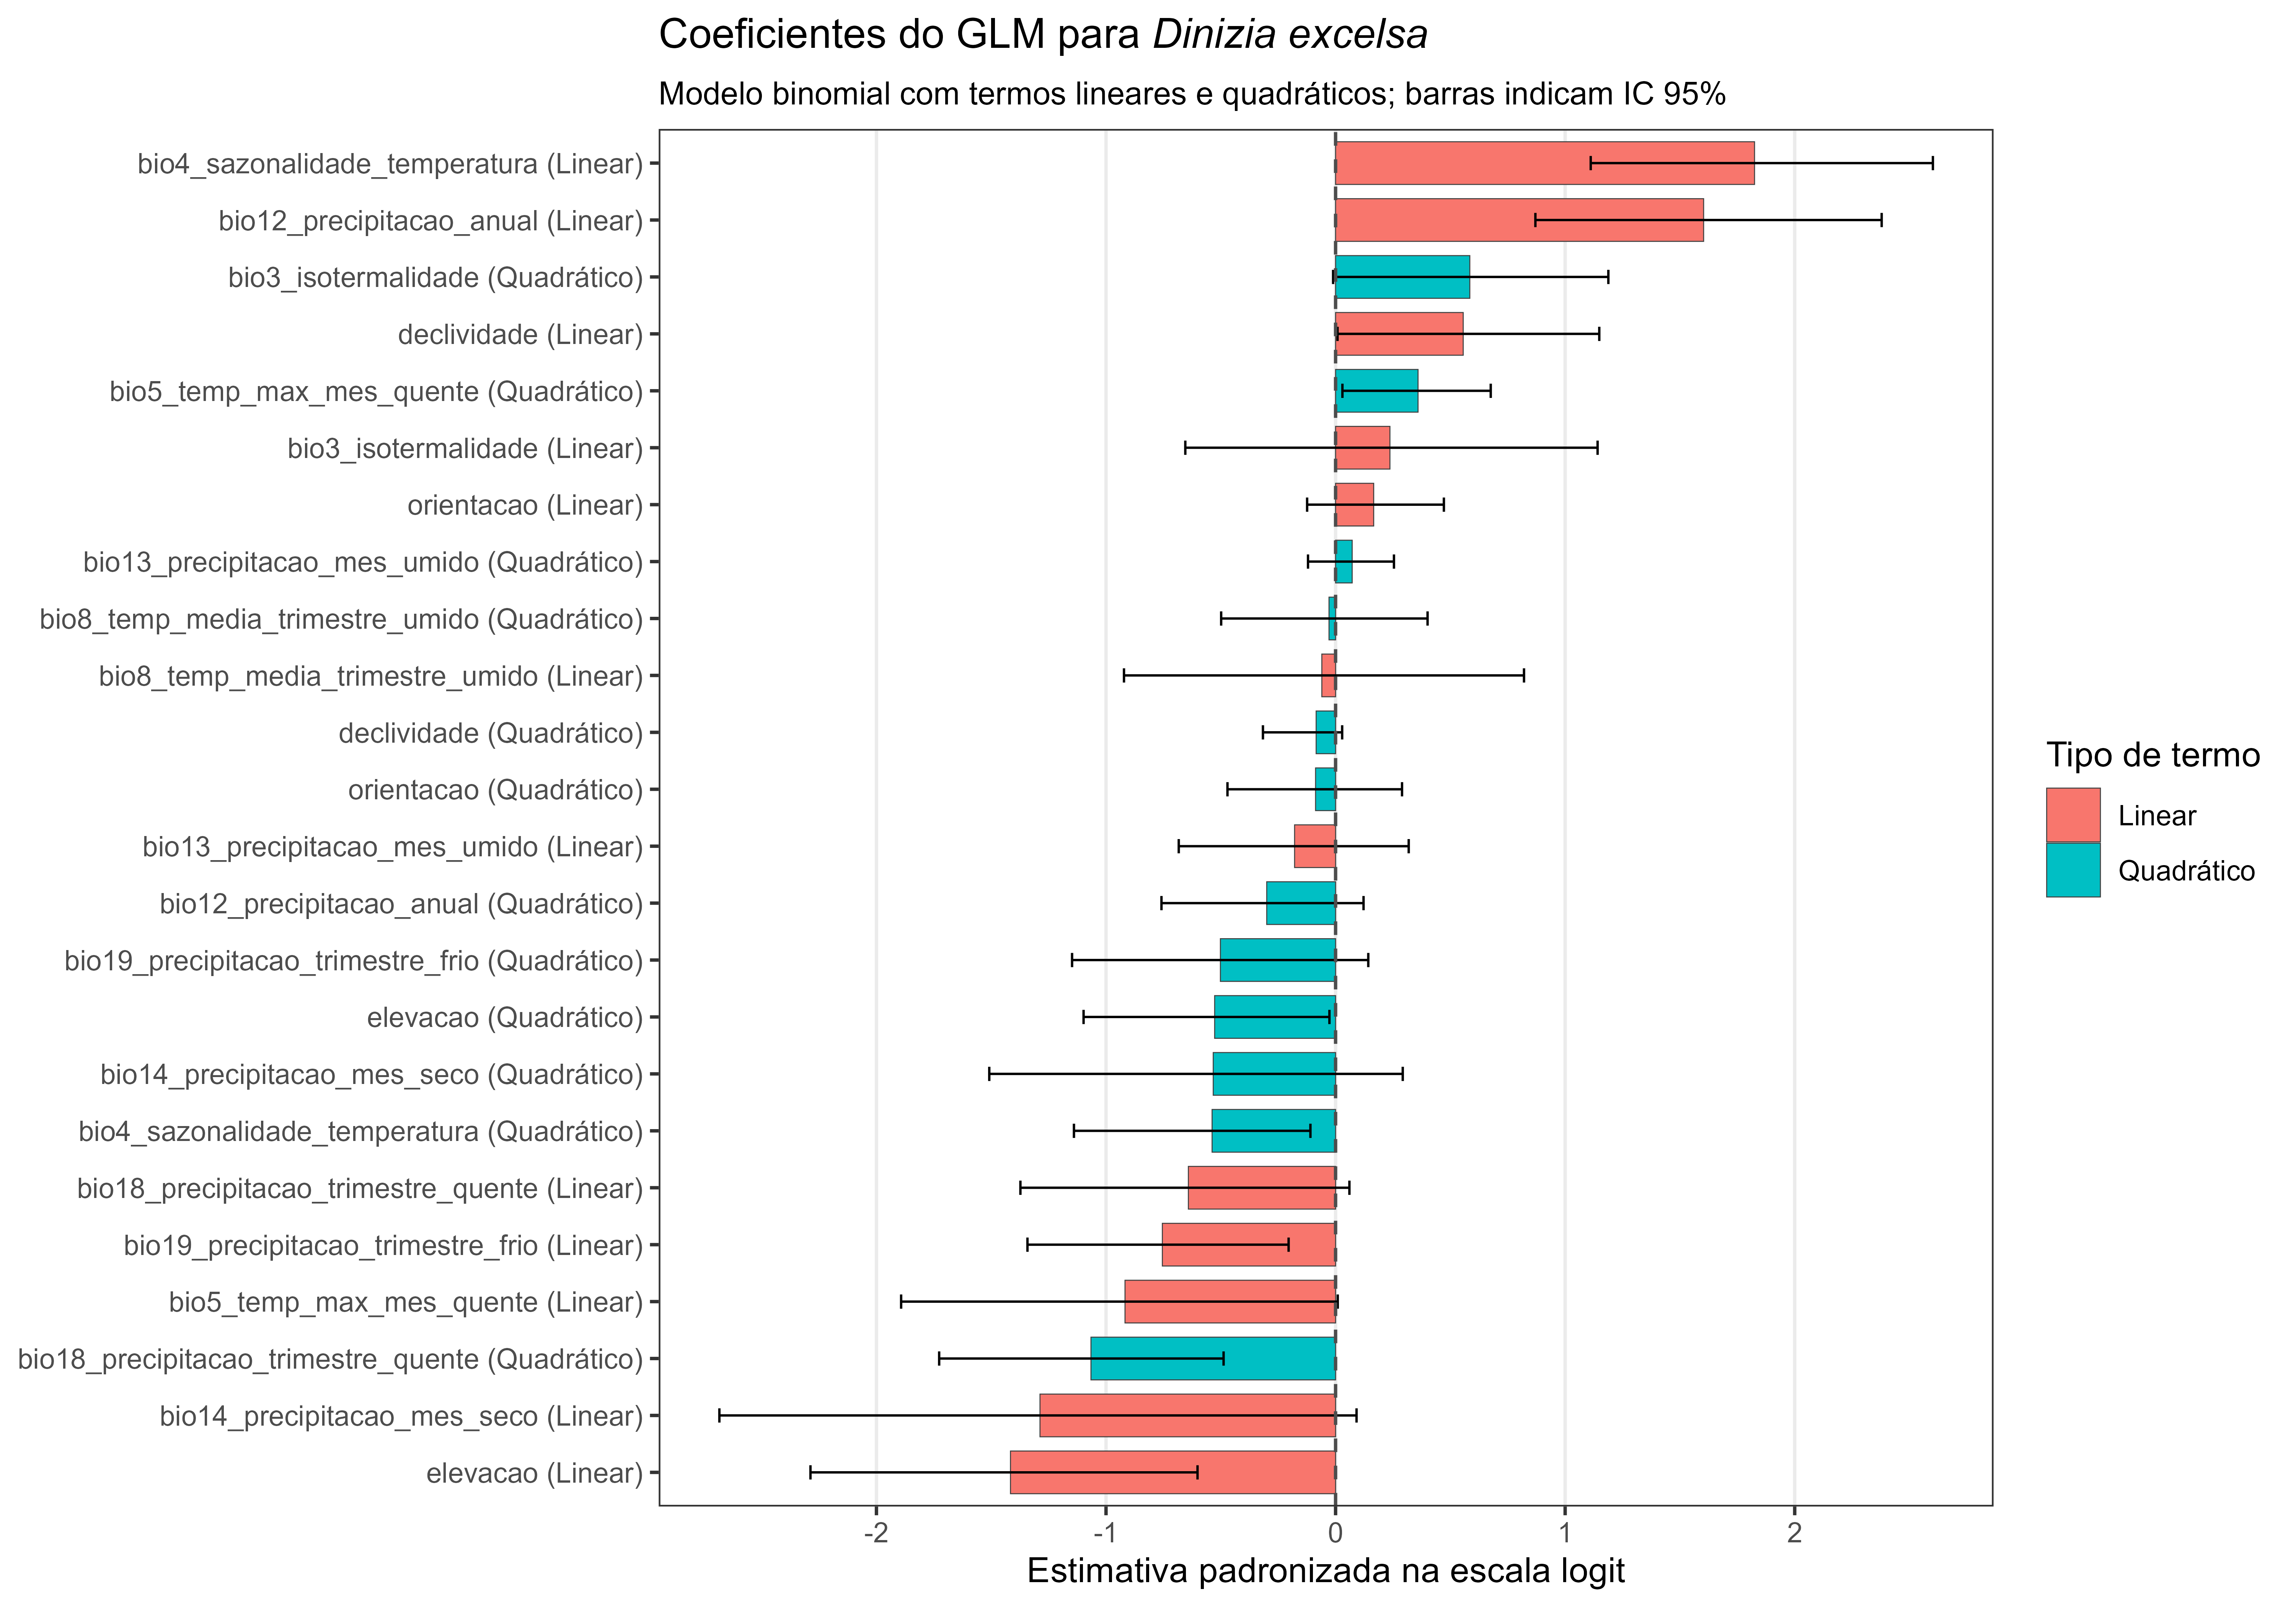
\includegraphics[width=0.88\textwidth]{figuras/unidade06/unidade06_coeficientes_glm.png}
  \caption{GLM coefficients estimated for \textit{Dinizia excelsa}. Conditional on the other model terms, positive values indicate positive associations with relative suitability and negative values indicate negative associations.}
  \label{fig:unidade06_coeficientes_glm}
\end{figure}

\section{Model Evaluation}

The GLM is evaluated using AUC, TSS, sensitivity, specificity, and a confusion
matrix. AUC summarizes discrimination across thresholds; TSS combines
sensitivity and specificity. With presence--background data, these metrics are
comparative indicators rather than absolute validation of the species' actual
distribution.

\rscriptfile{scripts/unidade06/04_avaliar_glm_dinizia.R}

\begin{figure}[H]
  \centering
  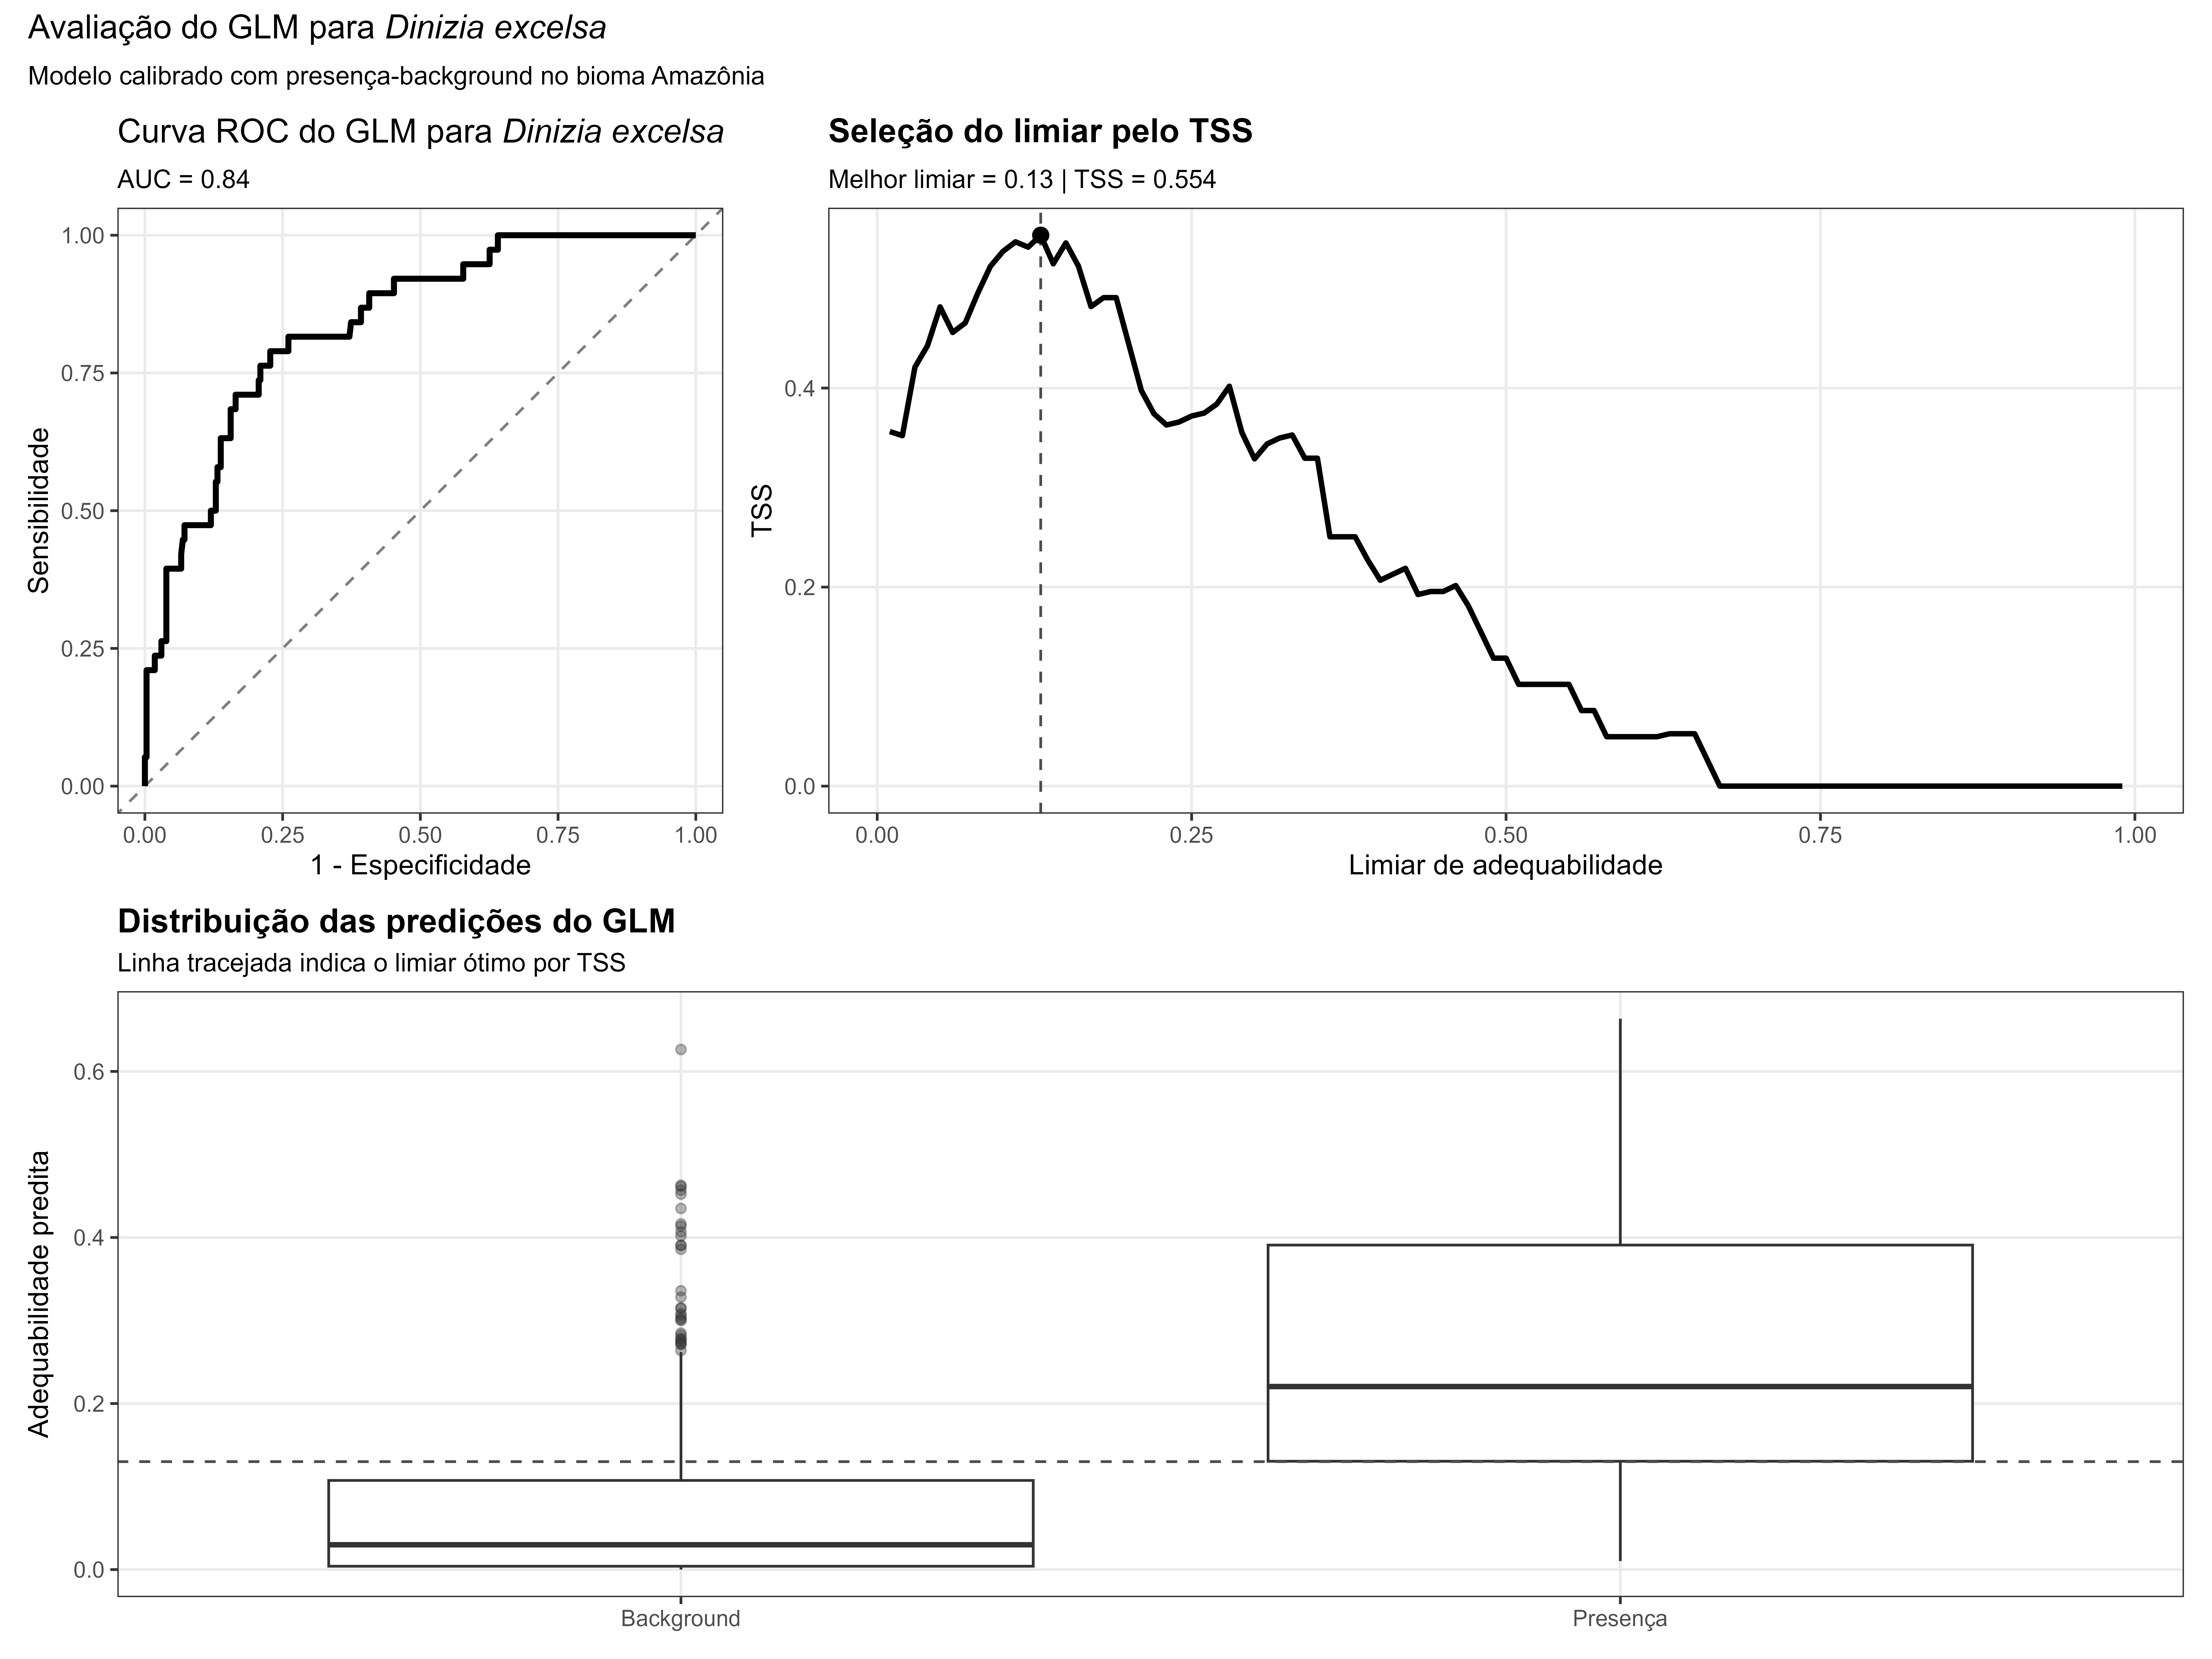
\includegraphics[width=0.82\textwidth]{figuras/unidade06/unidade06_avaliacao_glm_patchwork.png}
  \caption{ROC curve for the GLM fitted to \textit{Dinizia excelsa}.}
  \label{fig:unidade06_roc_glm}
\end{figure}

\section{Partial Response Curves}

Partial response curves show how estimated suitability changes along one
predictor while the others are held constant. They are essential for ecological
interpretation of model behavior.

\rscriptfile{scripts/unidade06/06_curvas_resposta_glm.R}

\begin{figure}[H]
  \centering
  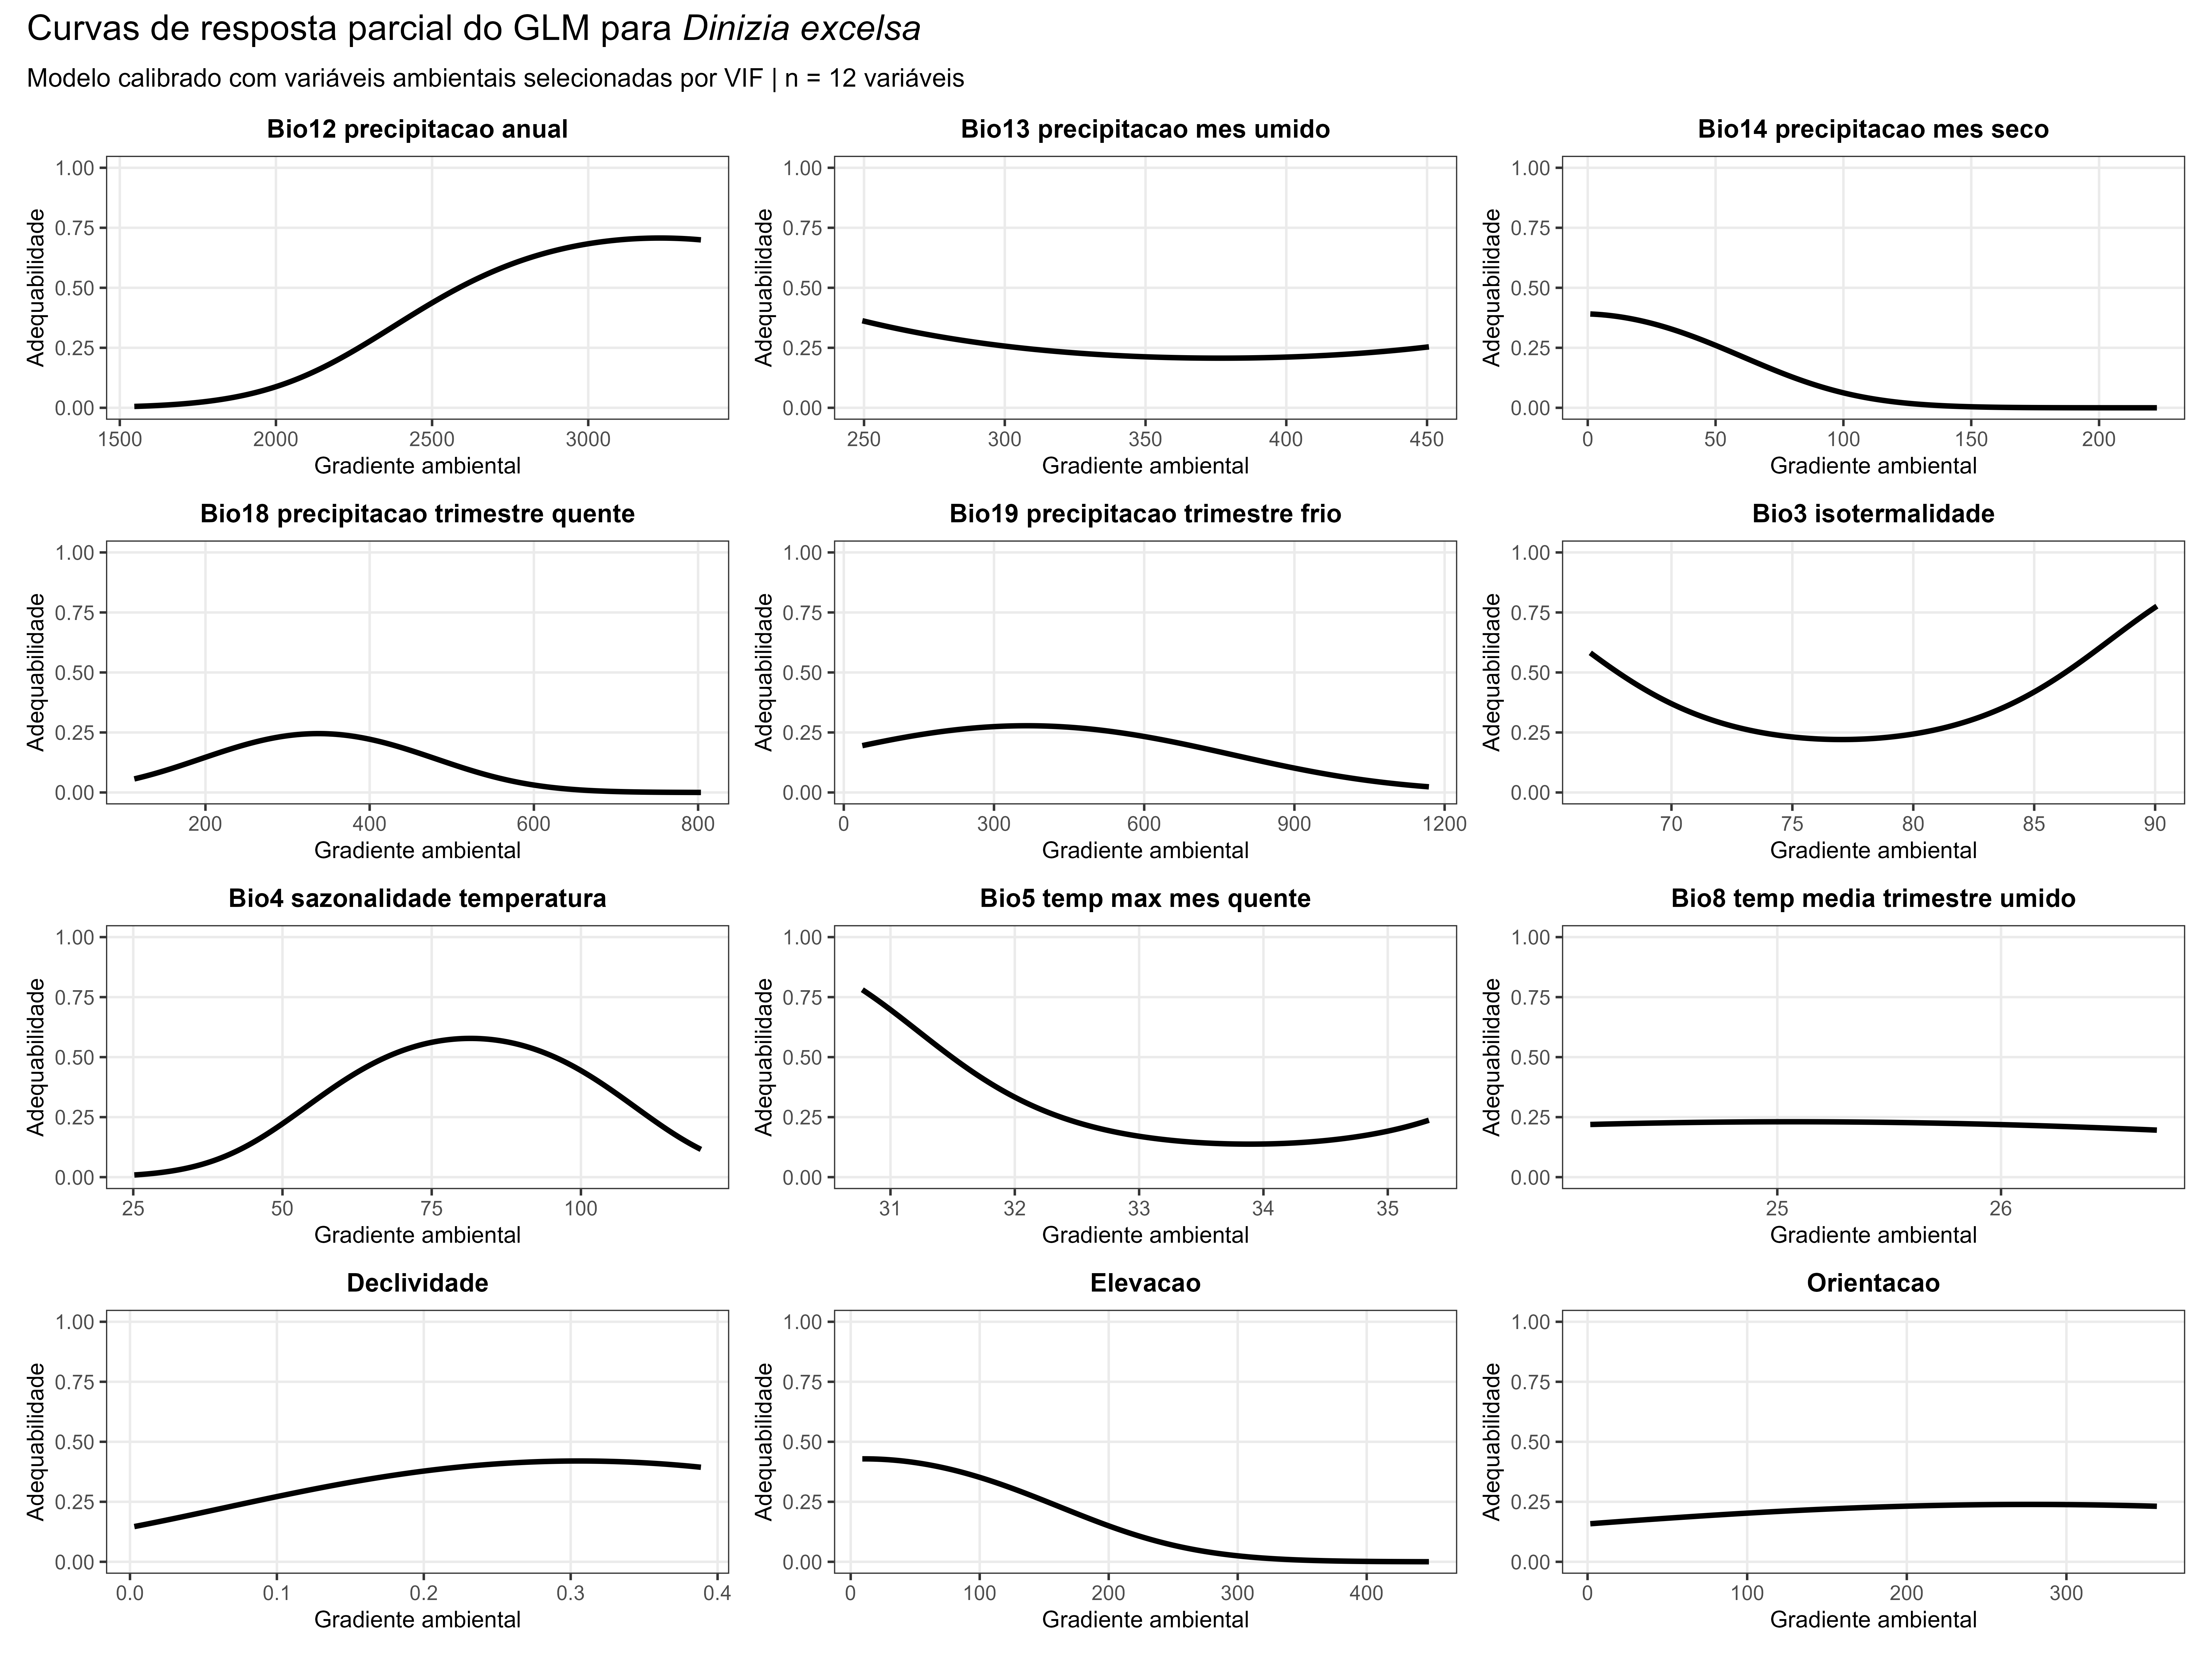
\includegraphics[width=0.96\textwidth]{figuras/unidade06/unidade06_curvas_resposta_glm.png}
  \caption{Partial response curves from the GLM for the selected environmental predictors.}
  \label{fig:unidade06_curvas_resposta}
\end{figure}

\section{Spatial Projection of Current Suitability}

After fitting and evaluation, the GLM is projected onto the environmental stack
for the study area, producing a continuous map of current environmental
suitability for \textit{Dinizia excelsa}.

\rscriptfile{scripts/unidade06/05_predicao_espacial_glm.R}

\begin{figure}[H]
  \centering
  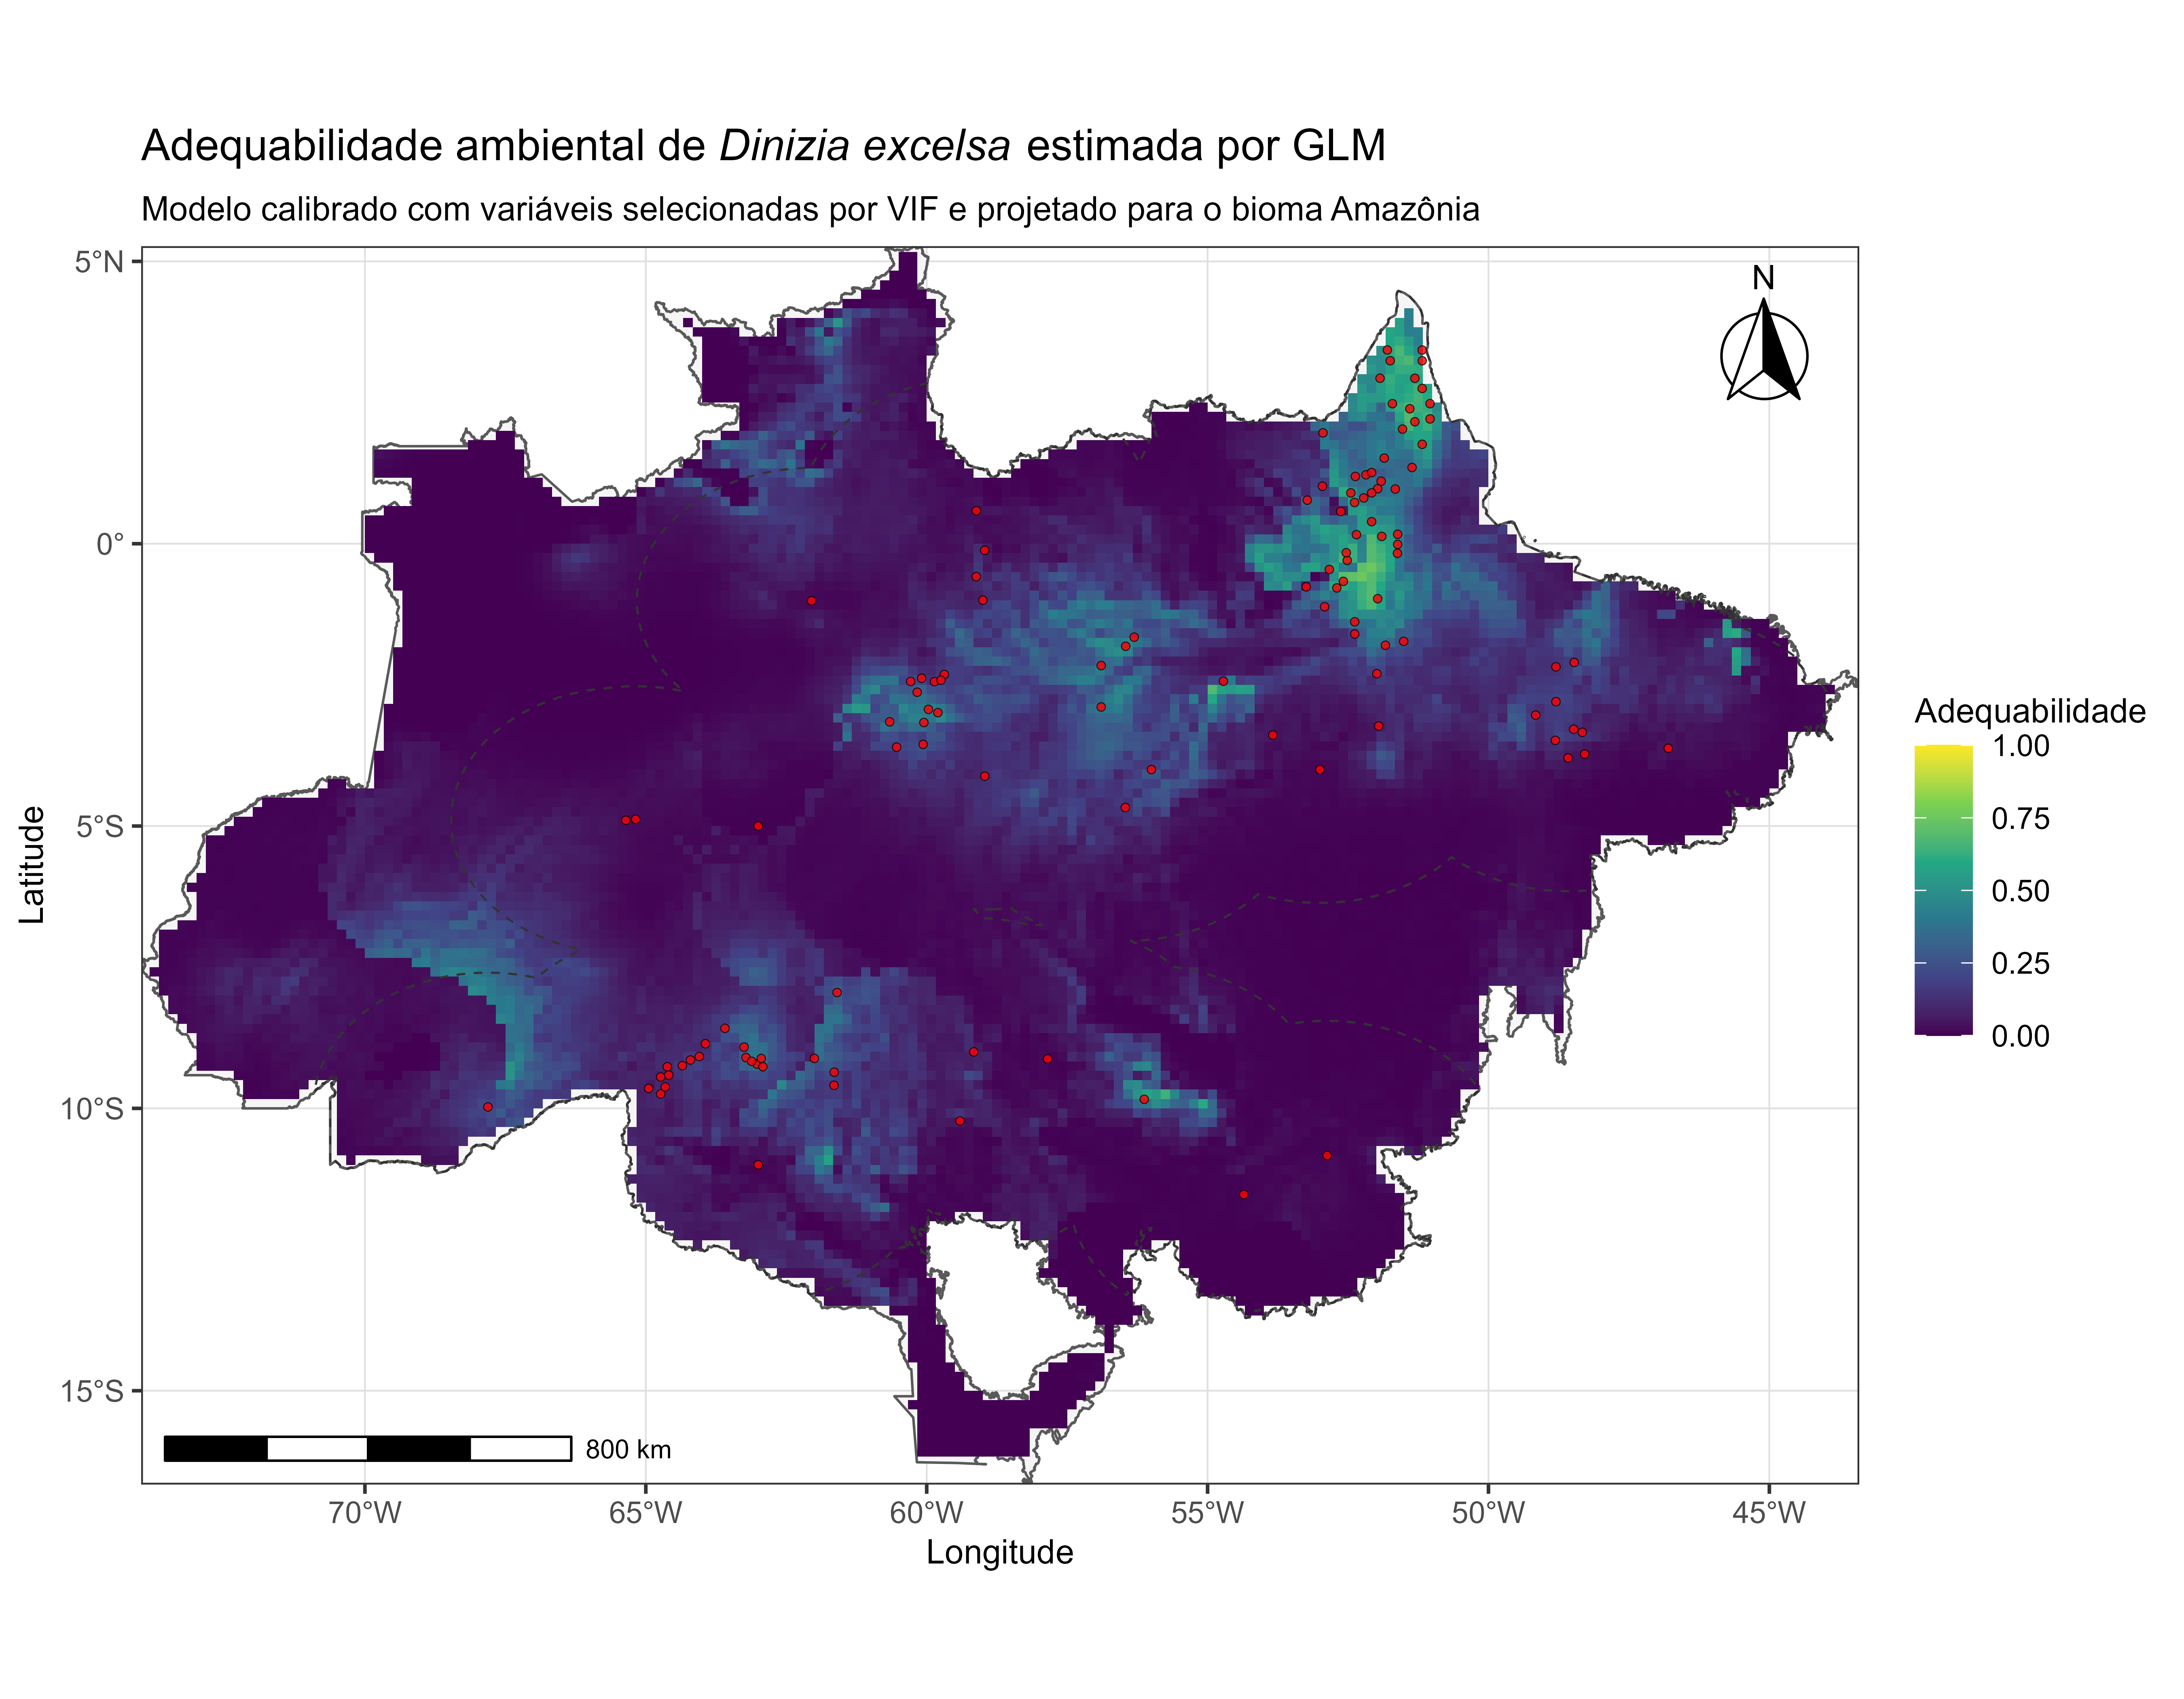
\includegraphics[width=0.90\textwidth]{figuras/unidade06/unidade06_adequabilidade_glm.png}
  \caption{Current environmental suitability for \textit{Dinizia excelsa} estimated with a GLM.}
  \label{fig:unidade06_adequabilidade_glm}
\end{figure}

\section{Complete Pipeline}
\rscriptfile{scripts/unidade06/07_pipeline_glm.R}

\section{Chapter Summary}

The GLM is a simple, interpretable, and robust starting point for SDM. Although
less flexible than GAM, Random Forest, BRT, or Maxent, it makes the relationship
between occurrence and environmental gradients explicit. It is consequently
valuable in teaching, exploratory analysis, and studies prioritizing
transparency and ecological interpretation.

\begin{conceito}[title={\faBook\quad Key message}]
The GLM bridges classical statistics and modern SDM: it is simple enough for
ecological interpretation but sufficiently powerful to produce suitability
maps when calibrated appropriately.
\end{conceito}

\section{Review Exercises}
\begin{enumerate}
  \item Why is the binomial family appropriate for presence--background models?
  \item What does the logit function represent in a GLM?
  \item Why are quadratic terms useful in SDM?
  \item Distinguish positive and negative GLM coefficients.
  \item Explain the difference between AUC and TSS.
  \item Why are partial response curves important for ecological interpretation?
  \item Which limitations should be considered when using GLMs for spatial projection?
\end{enumerate}
